\section{Bias-Variance Tradeoffs in Data with Binary Features}

Now, assume that \(\mat{X}\) and \(\vec{\beta}\) are fixed and that \(\vec{y} = \mat{X}\vec{\beta} + \vec{\varepsilon}\), where \(\varepsilon_i\) is identically and independently distributed noise with mean zero and finite variance \(\sigma_\varepsilon^2\). We are interested in the expected value of \Cref{eq:orthogonal-solution}. Let \(Z = \tilde{\vec{x}}_j^\T \vec{y} = \tilde{\vec{x}}_j^\T(\mat{X}\vec{\beta} + \vec{\varepsilon})\) and \(d_j = s_j\left(\tilde{\vec{x}}_j^\T \tilde{\vec{x}}_j + \lambda_2\right)\) so that \(\hat{\beta}_j = \st_{\lambda_1}(Z)/d_j\). We start by focusing on the numerator, since the denominator, \(d_j\), is fixed. First observe that
\[
  \E Z = \mu = \E \left( \tilde{\vec{x}}_j^\T (\vec{x}_j\beta_j + \vec{\varepsilon}) \right)  = \tilde{\vec{x}}_j^\T\vec{x}_j \beta_j.
\]
And for the variance, we have
\[
  \var Z = \sigma^2 = \var\left(\tilde{\vec{x}}_j ^\T \vec{\varepsilon}\right) = \sigma_\varepsilon^2 \lVert \tilde{\vec{x}}_j\rVert_2^2 .
\]

The expected value of the soft-thresholding estimator is
\begin{align}
  \label{eq:st-expected-value}
  \E \st_\lambda(Z) & = \int_{-\infty}^\infty \st_\lambda(z) f_Z(z) \du z                                                   \nonumber \\
                    & = \int_{-\infty}^\infty \ind{|z| > \lambda} (z -\sign(z)\lambda) f_Z(z) \du z                         \nonumber \\
                    & = \int_{-\infty}^{-\lambda}(z + \lambda)f_Z(z) \du z + \int_{\lambda}^\infty (z - \lambda)f_Z(z) \du z.
\end{align}
And then the bias of \(\hat\beta_j\) with respect to the true coefficient \(\beta_j^*\) is
\begin{equation}
  \label{eq:betahat-bias}
  \E \hat\beta_j - \beta_j^* = \frac{1}{d_j}\E \st_\lambda(Z) - \beta^*_j.
\end{equation}

Finally, we note that the variance of the soft-thresholding estimator is
\begin{equation}
  \label{eq:st-variance}
  \var {S_\lambda(Z)} = \int_{-\infty}^{-\lambda}(z + \lambda)^2f_Z(z) \du z + \int_{\lambda}^\infty (z - \lambda)^2 f_Z(z) \du z - \left(\E \st_\lambda(Z)\right)^2
\end{equation}
and that the variance of the elastic net estimator is therefore
\begin{equation}
  \label{eq:betahat-variance}
  \var \hat\beta_j = \frac{1}{d_j^2} \var \st_\lambda(Z).
\end{equation}

% \subsection{Normally Distributed Noise}

Next, we add the additional assumption that \(\vec{\varepsilon}\) is normally distributed. Then
\[
  Z \sim \normal\left(\tilde{\vec{x}}_j^\T\vec{x}_j \beta_j, \sigma_\varepsilon^2 \lVert \tilde{\vec{x}}_j\rVert_2^2 \right).
\]
Let \(\theta = -\mu -\lambda_1 \) and \(\gamma = \mu - \lambda_1\). Then the expected value of soft-thresholding of \(Z\) is
\begin{align}
  \E \st_{\lambda_1}(Z) & = \int_{-\infty}^\frac{\theta}{\sigma} (\sigma u - \theta) \pdf(u) \du u + \int_{-\frac{\gamma}{\sigma}}^\infty (\sigma u + \gamma) \pdf(u) \du u                                               \nonumber                      \\
                        & = -\theta \cdf\left(\frac{\theta}{\sigma}\right) - \sigma \pdf\left(\frac{\theta}{\sigma}\right) + \gamma \cdf\left(\frac{\gamma}{\sigma}\right) + \sigma \pdf\left(\frac{\gamma}{\sigma}\right) \label{eq:mean-centered-eval}
\end{align}
where \(\pdf(u)\) and \(\cdf(u)\) are the probability density and cumulative distribution functions of the standard normal distribution, respectively.

Next, we consider what the variance of the elastic net estimator looks like.
Starting with the first term on the left-hand side of \Cref{eq:st-variance}, we have
\begin{multline}
  \label{eq:mc-var-part1}
  \int_{-\infty}^{-\lambda_1}(z+ \lambda_1)^2 f_Z(z) \du z = \sigma^2 \int_{-\infty}^{\frac{\theta}{\sigma}} y^2 \pdf(y) \du y + 2 \theta \sigma \int_{-\infty}^{\frac{\theta}{\sigma}} y \pdf(y) \du y + \theta^2 \int_{-\infty}^{\frac{\theta}{\sigma}} \pdf(y) \du y \\
  = \frac{\sigma^2}{2} \left( \erf\left(\frac{\theta}{\sigma\sqrt{2}}\right) - \frac{\theta}{\sigma}\sqrt{\frac{2}{\pi}} \exp\left(-\frac{\theta^2}{2\sigma^2}\right) + 1 \right) + 2 \theta \sigma \pdf \left(\frac{\theta}{\sigma}\right) + \theta^2 \cdf\left(\frac{\theta}{\sigma}\right).
\end{multline}
Similar computations for the second term on the left-hand side of \Cref{eq:st-variance} yield
\begin{multline}
  \label{eq:mc-var-part2}
  \int_{\lambda_1}^{\infty}(z - \lambda_1)^2 f_Z(z) \du z \\
  = \frac{\sigma^2}{2} \left( \erf\left(\frac{\gamma}{\sigma\sqrt{2}}\right) - \frac{\gamma}{\sigma}\sqrt{\frac{2}{\pi}} \exp\left(-\frac{\gamma^2}{2\sigma^2}\right) + 1 \right) + 2 \gamma \sigma \pdf \left(\frac{\gamma}{\sigma}\right) + \gamma^2 \cdf\left(\frac{\gamma}{\sigma}\right).
\end{multline}
Plugging \Cref{eq:mean-centered-eval,eq:mc-var-part1,eq:mc-var-part2} into \Cref{eq:betahat-variance} yields the variance of the estimator. Consequently, we can also compute the mean-squared error via the bias-variance decomposition
\begin{equation}
  \label{eq:betahat-mse}
  \mse (\hat\beta_j, \beta^*_j) = \var\hat\beta_j + \left(\E \hat\beta_j - \beta^*_j\right)^2.
\end{equation}

% \subsubsection{Binary Features}

Our results have so far covered the general case where we have made no assumptions on \(\mat{X}\), except for being non-random. But our main focus in this paper
is the case when \(\vec{x_j}\) is a binary feature with class balance \(q\), that is, \(x_{ij} \in \{0, 1\}\) for all \(i\) and \(\sum_{i=1}^n x_{ij} = nq\).
In this case, we observe that
\[
  \begin{aligned}
    \tilde{\vec{x}}_j^\T \tilde{\vec{x}}_j & = \frac{1}{s_j^2}(\vec{x}_j - \ones c_j)^\T (\vec{x}_j - \ones c_j) = \frac{1}{s^2_j}(nq - 2nq^2 + nq^2) = \frac{nq(1-q)}{s^2_j}, \\
    \tilde{\vec{x}}_j^\T \vec{x}_j         & = \frac{1}{s_j}(\vec{x}_j^\T \vec{x}_j - \vec{x}_j^\T \ones c_j) = \frac{nq(1 - q)}{s_j}.
  \end{aligned}
\]
And consequently
\[
  \mu = \frac{\beta^*_j nq(1 - q)}{s_j}, \qquad \sigma^2 = \frac{\sigma_\varepsilon^2nq(1 - q)}{s^2_j}, \qquad d_j = \frac{nq(1 -q)}{s_j}  + \lambda_2 s_j.
\]
We will allow ourselves to abuse notation and overload the definitions of \(\mu\), \(\sigma^2\), and \(d_j\) as functions of \(q\). Then, an expression for the expected value of the elastic net estimate with respect to \(q\) can be obtained by plugging in \(\mu\) and \(\sigma\) into \Cref{eq:mean-centered-eval}.

We are mainly interested in examining the case when \(\vec{x}_j\) is imbalanced and what effect various approaches to normalizing the features
has on the elastic net estimator. In order to study this, we will parameterize the scaling factors \(s_j\) for \(j  \in [p]\) by \(s_j = (q - q^2)^\delta\), \(\delta \geq 0\).
This includes the cases that we are primary interested in, that is,
\begin{itemize}
  \item \(\delta = 0\): no scaling, which includes min--max and max--abs normalization,
  \item \(\delta = 1/2\): standardization, and
  \item \(\delta = 1\): scaling by the variance.
\end{itemize}
Note that the last of these cases does not correspond to a standard type of normalization. But as we will see, it has some interesting properties in the case of binary features.

A natual consequence of the normal distribution of \(Z\) is that the probability of selection in the elastic net problem is given by
\begin{align*}
  \Pr\left(\hat{\beta}_j \neq 0\right) & = \Pr\left(\st_{\lambda_1}(Z) \neq 0\right)                                                                                         \\
                                       & = \Pr\left(Z > \lambda_1\right) + \Pr\left(Z < -\lambda_1\right)                                                                    \\
                                       & = \cdf\left(\frac{\mu - \lambda_1}{\sigma}\right) + \cdf\left(\frac{- \mu -\lambda_1}{\sigma}\right).                               \\
                                       & = \cdf \left( \frac{\beta_j^*n (q-q^2)^{1/2} - \lambda_1(q-q^2)^{\delta - 1/2}}{\sigma_\varepsilon \sqrt{n}}\right)                 \\
                                       & \phantom{={}} + \cdf \left( \frac{-\beta_j^*n (q-q^2)^{1/2} - \lambda_1(q-q^2)^{\delta - 1/2}}{\sigma_\varepsilon \sqrt{n}}\right).
\end{align*}

Letting \(\theta = -\mu - \lambda_1 \) and \(\gamma = \mu - \lambda_1\), we can express the probability of selection in the limit as \(q \rightarrow 1^+\) as
\[
  \lim_{q \rightarrow 1^+} \Pr(\hat{\beta}_j \neq 0) =
  \begin{cases}
    0                                                                & \text{if } 0 \leq \delta < \frac{1}{2}, \\
    2\cdf\left(-\frac{\lambda_1}{\sigma_\varepsilon \sqrt{n}}\right) & \text{if } \delta = \frac{1}{2},        \\
    1                                                                & \text{if } \delta > \frac{1}{2}.
  \end{cases}
\]

\begin{figure}[htpb]
  \centering
  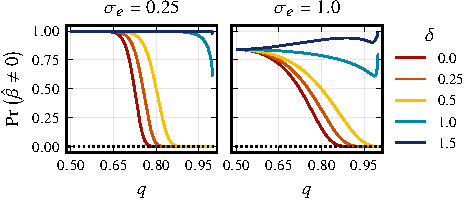
\includegraphics[]{plots/selection_probability.pdf}
  \caption{%
    Probability of selection in the elastic net problem given a measurement noise level \(\sigma_\varepsilon\), a regularization parameter \(\lambda_1\), and a class balance \(q\). The scaling factor is parameterized by \(s_j = (q - q^2)^\delta\), \(\delta \geq 0\). The dotted line represents the asymptotic limit for the standardization case, \(\delta = 1/2\). }
  \label{fig:selection-probability}
\end{figure}

In \Cref{thm:classbalance-bias}, we show what the
bias is under mean-centering and scaling with \(s_j = (q - q^2)^\delta\), \(\delta \geq 0\).

\begin{theorem}
  \label{thm:classbalance-bias}
  If \(\vec{x}_j\) is a binary feature with class balance \(q \in (0, 1)\), \(\lambda_1 \in (0,\infty)\), \(\lambda_2 \in [0,\infty)\), \(\sigma_\varepsilon > 0\), and \(s_j = (q - q^2)^{\delta}\), \(\delta \geq 0\)  then
  \[
    \lim_{q \rightarrow 1^+} \E \hat{\beta}_j =
    \begin{cases}
      0                                                                                                  & \text{if } 0 \leq \delta < \frac{1}{2}, \\
      \frac{2n \beta_j^*}{n + \lambda_2} \cdf\left(-\frac{\lambda_1}{\sigma_\varepsilon \sqrt{n}}\right) & \text{if } \delta = \frac{1}{2},        \\
      \beta^*_j                                                                                          & \text{if } \delta \geq 1.
    \end{cases}
  \]
\end{theorem}
\begin{proof}

  Since \(s_j = (q - q^2)^\delta\), we have
  \begin{align*}
    \mu    & = \beta_j^* n (q - q^2)^{1 - \delta}                     & \frac{\theta}{\sigma} & = -a \sqrt{q(1-q)} - b (q - q^2)^{\delta - 1/2},           \\
    \sigma & = \sigma_\varepsilon \sqrt{n} (q - q^2)^{1/2 - \delta},  & \frac{\gamma}{\sigma} & = a \sqrt{q(1-q)} - b (q - q^2)^{\delta - 1/2},            \\
    d_j    & = n (q - q^2)^{1 - \delta} + \lambda_2 (q - q^2)^\delta, & \frac{\theta}{d_j}    & = -\beta_j^* - \frac{\lambda_1 (q - q^2)^{\delta - 1}}{n}, \\
    \theta & = -\beta^*_j n (q - q^2)^{1-\delta} - \lambda_1,         & \frac{\gamma}{d_j}    & = \beta_j^* - \frac{\lambda_1 (q - q^2)^{\delta - 1}}{n},  \\
    \gamma & = \beta^*_j n (q - q^2)^{1-\delta} - \lambda_1,
  \end{align*}
  with
  \[
    a = \frac{\beta_j^* \sqrt{n}}{\sigma_\varepsilon} \qquad \text{and} \qquad b = \frac{\lambda_1}{\sigma_\varepsilon \sqrt{n}}.
  \]

  We are interested in
  \begin{equation}
    \label{eq:eval-qlimit}
    \lim_{q \rightarrow 1^+} \E \hat{\beta}_j =\lim_{q \rightarrow 1^+}\frac{1}{d}\left(-\theta \cdf\left(\frac{\theta}{\sigma}\right) - \sigma \pdf\left(\frac{\theta}{\sigma}\right) + \gamma \cdf\left(\frac{\gamma}{\sigma}\right) + \sigma \pdf\left(\frac{\gamma}{\sigma}\right)\right).
  \end{equation}
  Before we proceed, note the following limits, which we will make repeated use of throughout the proof.
  \begin{equation}
    \label{eq:eval-sigma-limits}
    \lim_{q \rightarrow 1^+} \frac{\theta}{\sigma} = \lim_{q \rightarrow 1^+} \frac{\gamma}{\sigma} =
    \begin{cases}
      -\infty & \text{if } 0 \leq \delta < \frac{1}{2}, \\
      -b      & \text{if } \delta = \frac{1}{2},        \\
      0       & \text{if } \delta > \frac{1}{2},
    \end{cases}
  \end{equation}

  Starting with the terms involving \(\cdf\) inside the limit in \Cref{eq:eval-qlimit}, for now assuming that they are well-defined and that the limits of the remaining terms also exist seperately, we have
  \begin{align}
     & \lim_{q \rightarrow 1^+} \left(-\frac{\theta}{d} \cdf\left(\frac{\theta}{\sigma}\right) + \frac{\gamma}{d_j} \cdf \left(\frac{\gamma}{\sigma}\right)\right)                                                                                                                                                                                      \nonumber                                                        \\
     & = \lim_{q \rightarrow 1^+} \Bigg(\left(\frac{\beta_j^* n}{n + \lambda_2 (q-q^2)^{2\delta - 1}} + \frac{\lambda_1}{n(q-q^2)^{1-\delta} + \lambda_2 (q-q^2)^{\delta}} \right) \cdf \left(\frac{\theta}{\sigma}\right)  \nonumber                                                                                                                                                                                    \\
     & \phantom{= \lim_{q \rightarrow 1^+} \Bigg( } + \left(\frac{\beta_j^* n}{n + \lambda_2 (q-q^2)^{2\delta - 1}} - \frac{\lambda_1}{n(q-q^2)^{1-\delta} + \lambda_2 (q-q^2)^{\delta}} \right)\cdf \left(\frac{\gamma}{\sigma}\right) \Bigg) \nonumber                                                                                                                                                                 \\
     & = \lim_{q \rightarrow 1^+} \frac{\beta_j^*n}{n + \lambda_2 (q-q^2)^{2\delta - 1}}\left(\cdf \left(\frac{\theta}{\sigma}\right) + \cdf \left(\frac{\gamma}{\sigma}\right) \right)                                                                                                                                                                                                                        \nonumber \\
     & \phantom{={}} +  \lim_{q \rightarrow 1^+}\frac{\lambda_1}{n(q-q^2)^{1-\delta} + \lambda_2(q -q^2)^{\delta}} \left(\cdf \left(\frac{\theta}{\sigma}\right) - \cdf \left(\frac{\gamma}{\sigma}\right)\right). \label{eq:eval-qlimit-terms}
  \end{align}
  Considering the first term in \Cref{eq:eval-qlimit-terms}, we see that
  \[
    \lim_{q \rightarrow 1^+} \frac{\beta_j^*n}{n + \lambda_2 (q-q^2)^{2\delta - 1}}\left(\cdf \left(\frac{\theta}{\sigma}\right) + \cdf \left(\frac{\gamma}{\sigma}\right) \right)  =
    \begin{cases}
      0                                            & \text{if } 0 \leq \delta < 1/2, \\
      \frac{2n \beta_j^*}{n + \lambda_2} \cdf (-b) & \text{if } \delta = 1/2,        \\
      \beta_j^*                                    & \text{if } \delta > 1/2.
    \end{cases}
  \]
  For the second term in \Cref{eq:eval-qlimit-terms}, we start by observing that if
  \(\delta = 1\), then \(q(1-q)^{\delta - 1} = 1\), and if \(\delta > 1\), then \(\lim_{q\rightarrow 1^+}(q - q^2)^{\delta - 1} = 0\). Moreover, the arguments of \(\cdf\) approach 0 in the limit for \(\delta \geq 1\), which means that the entire term vanishes in both cases (\(\delta \geq 1\)).

  For \(0 \leq \delta < 1\), the limit is indeterminite of the form \(\infty \times 0\). We define
  \[
    f(q) = \cdf \left(\frac{\theta}{\sigma}\right) - \cdf \left(\frac{\gamma}{\sigma}\right)
    \qquad\text{and}\qquad
    g(q) = n(q - q^2)^{1-\delta} + \lambda_2(q - q^2)^\delta,
  \]
  such that we can express the limit as \(\lim_{q \rightarrow 1^+}f(q)/g(q)\). The corresponding derivatives are
  \[
    \begin{aligned}
      f'(q) & = \left(-\frac{a}{2}(1-2q)(q - q^2)^{-1/2} - b(\delta - 1/2)(1-2q)(q - q^2)^{\delta - 3/2}\right)\pdf\left(\frac{\theta}{\sigma}\right)                 \\
            & \phantom{= {}} - \left(-\frac{a}{2}(1-2q)(q - q^2)^{-1/2} - b(\delta - 1/2)(1-2q)(q - q^2)^{\delta - 3/2}\right)\pdf\left(\frac{\gamma}{\sigma}\right), \\
      g'(q) & = n(1 - \delta)(1-2q)(q - q^2)^{-\delta} + \lambda_2 \delta(1 - 2q) (q - q^2)^{\delta - 1}
    \end{aligned}
  \]
  Note that \(f(q)\) and \(g(q)\) are both differentiable and \(g'(q) \neq 0\) everywhere in the interval \((1/2, 1)\). Now note that we have
  \begin{multline}
    \label{eq:eval-qlimit-secondterm}
    \frac{f'(q)}{g'(q)} = \frac{1}{n(1-\delta)(q-q^2)^{1/2-\delta} + \lambda_2 \delta (1-2q)(q - q^2)^{\delta-1/2}} \\
    \times \left(\left(-\frac{a}{2} - b(\delta - 1/2)(q - q^2)^{\delta - 1}\right)\pdf\left(\frac{\theta}{\sigma}\right) - \left(\frac{a}{2} - b(\delta - 1/2)(q - q^2)^{\delta - 1}\right)\pdf\left(\frac{\gamma}{\sigma}\right) \right).
  \end{multline}
  For \(0 \leq \delta < 1/2\), $\lim_{q \rightarrow 1^+}f'(q)/g'(q) = 0$ since the exponential terms of \(\pdf\) in \Cref{eq:eval-qlimit-secondterm} dominate in the limit.

  For \(\delta = 1/2\), we have
  \[
    \lim_{q \rightarrow 1^+} \frac{f'(q)}{g'(q)} = -\frac{a}{n + \lambda_2} \lim_{q \rightarrow 1^+}\left(\pdf\left(\frac{\theta}{\sigma}\right) + \pdf\left(\frac{\gamma}{\sigma}\right)\right) = -\frac{a}{n + \lambda_2} \pdf(-b)
  \]
  so that we can use L'Hôpital's rule to show that the second term in \Cref{eq:eval-qlimit-terms} becomes
  \begin{equation}
    \label{eq:eval-qlimit-stdcase}
    -\frac{2\beta_j^*\lambda_1\sqrt{n}}{\sigma_\varepsilon(n + \lambda_2)} \pdf\left(\frac{-\lambda_1}{\sigma_\varepsilon\sqrt{n}}\right).
  \end{equation}

  For \(\delta > 1/2\), we have
  \[
    \begin{aligned}
      \lim_{q \rightarrow 1^+} \frac{f'(q)}{g'(q)} & = \lim_{q \rightarrow 1^+} \frac{-\frac{a}{2}\left(\pdf\left(\frac{\theta}{\sigma}\right) + \pdf\left(\frac{\gamma}{\sigma}\right)\right)}{n(1-\delta)(q - q^2)^{1/2 - \delta} + \lambda_2 \delta(1 - 2q)(q - q^2)^{\delta - 1/2}}                                                       \\
                                                   & \phantom{= {}} + \lim_{q \rightarrow 1^+} \frac{b(\delta - 1/2)\left(\pdf\left(\frac{\gamma}{\sigma}\right) - \pdf\left(\frac{\theta}{\sigma}\right)\right)}{n(1 - \delta)(q - q^2)^{3/2 - 2\delta} + \lambda_2 \delta (1 - 2q)(q - q^2)^{1/2}}                                          \\
                                                   & = 0 + \lim_{q \rightarrow 1^+} \frac{b(\delta - 1/2) e^{-\frac{1}{2}\left(a^2(q - q^2) + b^2(q - q^2)^{2\delta - 1}\right)}\left(e^{-ab(q-q^2)^\delta} - e^{ab(q-q^2)^\delta}\right)}{\sqrt{2\pi}\left(n(1-\delta)(q - q^2)^{3/2 - 2\delta} + \lambda_2\delta(1-2q)(q-q^2)^{1/2}\right)} \\
                                                   & = 0
    \end{aligned}
  \]
  since the exponential term in the numerator dominates.

  Now we proceed to consider the terms involving \(\pdf\) in \Cref{eq:eval-qlimit}. We have
  \begin{equation}
    \label{eq:eval-qlimit-pdfterm}
    \lim_{q \rightarrow 1^+} \frac{\sigma}{d} \left(\pdf \left(\frac{\gamma}{\sigma}\right) - \pdf \left(\frac{\theta}{\sigma}\right)\right)
    = \sigma_\varepsilon \sqrt{n} \lim_{q \rightarrow 1^+} \frac{ \pdf\left(\frac{\gamma}{\sigma}\right) - \pdf\left(\frac{\theta}{\sigma}\right)}{n(q-q^2)^{1/2} + \lambda_2(q - q^2)^{2\delta - 1/2}}
  \end{equation}
  For \(0 \leq \delta < 1/2\), we observe that the exponential terms in \(\pdf\) dominate in the limit, and so we can distribute the limit and consider the limits of the respective terms individually, which both vanish.

  For \(\delta \geq 1/2\), the limit in \Cref{eq:eval-qlimit-pdfterm} has an indeterminate form of the type \(\infty \times 0\). Define
  \[
    u(q) = \pdf\left(\frac{\gamma}{\sigma}\right) - \pdf\left(\frac{\theta}{\sigma}\right)
    \qquad\text{and}\qquad
    v(q) = n(q - q^2)^{1/2} + \lambda_2 (q - q^2)^{2\delta - 1/2}
  \]
  which are both differentiable in the interval \((1/2, 1)\) and \(v'(q) \neq 0\) everywhere in this interval. The derivatives are
  \[
    \begin{aligned}
      u'(q) & = -\pdf\left(\frac{\gamma}{\sigma}\right)\frac{\gamma}{\sigma} \left(\frac{1}{2}\left(a(1-2q)(q - q^2)^{-1/2}\right) - b(\delta - 1/2)(1- 2q)(q - q^2)^{\delta - 3/2}\right)                  \\
            & \phantom{= {}} + \pdf\left(\frac{\theta}{\sigma}\right) \frac{\theta}{\sigma} \left(-\frac{1}{2}\left(a(1-2q)(q - q^2)^{-1/2}\right) - b(\delta - 1/2)(1- 2q)(q - q^2)^{\delta - 3/2}\right), \\
      v'(q) & = \frac{n}{2} (1 - 2q)(q - q^2)^{-1/2} + \lambda_2(2\delta - 1/2)(1 - 2q)(q - q^2)^{2\delta - 3/2}.
    \end{aligned}
  \]
  And so
  \begin{equation}
    \begin{split}
      \frac{u'(q)}{v'(q)} = \frac{1}{n + \lambda_2(4\delta - 1)(q - q^2)^{2\delta - 1}}  \Bigg( & -\left(a - b(2\delta - 1)(q - q^2)^{\delta - 1}\right) \pdf\left(\frac{\gamma}{\sigma}\right) \frac{\gamma}{\sigma} \\ & - \left(a + b(2\delta - 1)(q - q^2)^{\delta - 1}\right)\pdf\left(\frac{\theta}{\sigma}\right) \frac{\theta}{\sigma}\Bigg).
    \end{split}
  \end{equation}
  Taking the limit, rearranging, and assuming that the limits of the separate terms exist, we obtain
  \begin{multline}
    \label{eq:eval-qlimit-pdfterm-split}
    \lim_{q \rightarrow 1^+} \frac{u'(q)}{v'(q)} = - a \lim_{q \rightarrow 1^+}  \frac{1}{n + \lambda_2 (4 \delta - 1)(q - q^2)^{2\delta - 1}} \left( \pdf\left(\frac{\gamma}{\sigma}\right)\frac{\gamma}{\sigma} + \pdf\left(\frac{\theta}{\sigma}\right)\frac{\theta}{\sigma}\right) \\
    + b (2\delta - 1) \lim_{q \rightarrow 1^+} \frac{1}{n + \lambda_2 (4 \delta - 1)(q - q^2)^{2\delta - 1}} \bigg( \pdf\left(\frac{\gamma}{\sigma}\right) \left(a(q -q^2)^{\delta - 1/2}- b(q - q^2)^{2\delta - 3/2} \right) \\
    - \pdf\left(\frac{\theta}{\sigma}\right) \left(-a(q - q^2)^{\delta - 1/2} - b(q - q^2)^{2\delta - 3/2}\right) \bigg).
  \end{multline}
  For \(\delta = 1/2\), we have
  \[
    \lim_{q \rightarrow 1^+} \frac{u'(q)}{v'(q)} = -\frac{a}{n + \lambda_2}\left(-b \pdf(-b) - b \pdf(-b)\right) + 0 = 2ab \pdf(-b) = \frac{2 \beta_j^* \lambda_1}{\sigma_\varepsilon^2(n + \lambda_2)} \pdf \left(\frac{-\lambda_1}{\sigma_\varepsilon\sqrt{n}}\right).
  \]
  Using L'Hôpital's rule, the second term in \Cref{eq:eval-qlimit-pdfterm} must consequently be
  \[
    \frac{2 \beta_j^* \lambda_1\sqrt{n}}{\sigma_\varepsilon(n + \lambda_2)} \pdf \left(\frac{-\lambda_1}{\sigma_\varepsilon\sqrt{n}}\right).
  \]
  which cancels with \Cref{eq:eval-qlimit-stdcase}.

  For \(\delta > 1/2\), we first observe that the first term in \Cref{eq:eval-qlimit-pdfterm-split} tends to zero due to \Cref{eq:eval-sigma-limits} and
  the properties of the standard normal distribution. For the second term, we note that this is essentially
  of the same form as \Cref{eq:eval-qlimit-secondterm} and that the limit is therefore 0 here.
\end{proof}

\begin{corollary}[Bias in Ridge Regression]
  Asume the conditions of \Cref{thm:classbalance-bias} but that \(\lambda_1 = 0\). Then
  \[
    \lim_{q \rightarrow 1^+} \E \hat{\beta}_j =
    \begin{cases}
      0                                         & \text{if } 0 \leq \delta < 1/2, \\
      \frac{\beta_j^*}{1 + \frac{\lambda_2}{n}} & \text{if } \delta = 1/2,        \\
      0                                         & \text{if } \delta > 1/2.
    \end{cases}
  \]
\end{corollary}
\begin{proof}
  If \(\lambda_1 = 0\), we have \(\E \st_{\lambda_1}(Z) = \mu\) and consequently
  \[
    \E \hat{\beta}_j = \frac{\beta_j^*}{1 + \frac{\lambda_2}{n} (q - q^2)^{2\delta - 1}}.
  \]
  Then
  \[
    \lim_{q \rightarrow 1^+} \E \hat{\beta}_j = \frac{\beta_j^*}{1 + \frac{\lambda_2}{n}\lim_{q \rightarrow 1^+} (q - q^2)^{2\delta - 1}}.
  \]
  The result follows by noting that
  \[
    \lim_{q \rightarrow 1^+} (q - q^2)^{2\delta - 1} =
    \begin{cases}
      \infty    & \text{if } 0 \leq \delta < 1/2, \\
      1         & \text{if } \delta = 1/2,        \\
      \beta_j^* & \text{if } \delta > 1/2.
    \end{cases}
  \]
\end{proof}

\Cref{thm:classbalance-bias} shows that the bias of the elastic net estimator when \(0 \leq \delta < 1/2\), which includes to the case of min--max and max--abs normalization (no scaling), approaches
\(-\beta_j^*\) as \(q \rightarrow 1^+\). When \(\delta = 1/2\) (standardization), the lasso estimate does not vanish completely. Instead, it approaches the
true coefficient scaled by the probability that a standard normal variable is smaller than \(\beta_j^*\sqrt{n}\sigma_\varepsilon^{-1}\). For \(\delta \geq 1\), the
estimate is unbiased asymptotically. The last fact may seem somewhat counterintuitive but is a consequence of the variance of the distribution of the estimator exploding as \(q \rightarrow 1^+\).

\begin{theorem}
  \label{thm:classbalance-variance}
  If \(\vec{x}_j\) is a binary feature with class balance \(q \in (0, 1)\) and \(\lambda_1,\lambda_2 \in (0,\infty)\), \(\sigma_\varepsilon > 0\), and \(s_j = (q - q^2)^{\delta}\), \(\delta \geq 0\), then
  \[
    \lim_{q \rightarrow 1^+} \var \hat{\beta}_j =
    \begin{cases}
      0      & \text{if } 0 \leq \delta < \frac{1}{2}, \\
      \infty & \text{if } \delta \geq \frac{1}{2}.
    \end{cases}
  \]
\end{theorem}
\begin{proof}
  The variance of the elastic net estimator is given by
  \begin{multline}
    \label{eq:varthm-var}
    \var \hat{\beta}_j = \frac{1}{d^2}\Bigg( \frac{\sigma^2}{2}\bigg(2 + \erf\left(\frac{\theta}{\sigma \sqrt{2}}\right) - \frac{\theta}{\sigma}\sqrt{\frac{2}{\pi}} \exp\left(-\frac{\theta^2}{2\sigma^2}\right) + \erf\left(\frac{\gamma}{\sigma\sqrt{2}}\right) - \frac{\gamma}{\sigma} \sqrt{\frac{2}{\pi}} \exp\left(- \frac{\gamma^2}{2\gamma^2}\right)\bigg) \\
    + 2\theta\sigma \pdf\left(\frac{\theta}{\sigma}\right) + \theta^2 \cdf\left(\frac{\theta}{\sigma}\right) + 2\gamma \sigma \pdf\left(\frac{\gamma}{\sigma}\right) + \gamma^2 \cdf\left(\frac{\gamma}{\sigma}\right) \Bigg)
    - \left(\frac{1}{d}\E \hat{\beta}_j\right)^2.
  \end{multline}
  We start by noting the following identities:
  \[
    \begin{aligned}
      \theta^2                  & = \left(\beta_j^* n\right)^2 (q-q^2)^{2-2\delta} + \lambda_1^2 + 2\lambda_1 \beta_j^* n(q-q^2)^{1-\delta},              \\
      d^2                       & = n^2(q -q^2)^{2 - 2\delta} + 2n\lambda_2 (q-q^2) + \lambda_2^2 (q-q^2)^{2\delta},                                      \\
      \theta \sigma             & =  -\sigma_\varepsilon\left(\beta_j^* n^{3/2}(q- q^2)^{3/2-2\delta} + \sqrt{n} \lambda_1 (q-q^2)^{1/2 - \delta}\right), \\
      \frac{\theta^2}{\sigma^2} & = a^2(q-q^2) + b^2(q-q^2)^{2\delta - 1} + 2ab (q -q^2)^\delta,                                                          \\
      \frac{\sigma}{d}          & = \frac{\sigma_\varepsilon \sqrt{n}}{n(q-q^2)^\frac{1}{2} + \lambda_2 (q-q^2)^{2\delta - 1/2}}.
    \end{aligned}
  \]
  Expansions involving \(\gamma\), instead of \(\theta\), have identical expansions up to sign changes of the individual terms.
  Also recall the definitions provided in the proof of \Cref{thm:classbalance-bias}.

  Starting with the case when \(0 \leq \delta < 1/2\), we write the limit of \Cref{eq:varthm-var} as
  \begin{align*}
     & \lim_{q \rightarrow }\var \hat{\beta}_j                                                                                                                                                                                                                                                                                                                                             \\
     & = \sigma_\varepsilon^2 n  \lim_{q \rightarrow 1^+} \frac{1}{\left(n(q-q^2)^{1/2} + \lambda_2(q-q^2)^{2\delta - 1/2}\right)^2}\bigg(1 + \erf\left(\frac{\theta}{\sigma \sqrt{2}}\right) - \frac{\theta}{\sigma}\sqrt{\frac{2}{\pi}} \exp\left(-\frac{\theta^2}{2\sigma^2}\right)\bigg)                                                                                               \\
     & \phantom{= {}} + \sigma_\varepsilon^2 n  \lim_{q \rightarrow 1^+} \frac{1}{\left(n(q-q^2)^{1/2} + \lambda_2(q-q^2)^{2\delta - 1/2}\right)^2}\bigg(1 + \erf\left(\frac{\gamma}{\sigma\sqrt{2}}\right) - \frac{\gamma}{\sigma} \sqrt{\frac{2}{\pi}} \exp\left(- \frac{\gamma^2}{2\sigma^2}\right)\bigg)                                                                               \\
     & \phantom{= {}}+ \lim_{q \rightarrow 1^+} \frac{2\theta\sigma}{d^2} \pdf\left(\frac{\theta}{\sigma}\right) + \lim_{q \rightarrow 1^+} \frac{\theta^2}{d^2} \cdf\left(\frac{\theta}{\sigma}\right) + \lim_{q \rightarrow 1^+} \frac{2\gamma}{d^2} \sigma \pdf\left(\frac{\gamma}{\sigma}\right) + \lim_{q \rightarrow 1^+}\frac{\gamma^2}{d^2} \cdf\left(\frac{\gamma}{\sigma}\right) \\
     & \phantom{= {}}- \left( \lim_{q\rightarrow 1^+}\frac{1}{d}\E \hat{\beta}_j\right)^2,
  \end{align*}
  assuming, for now, that all limits exist. Next, let
  \[
    \begin{aligned}
      f_1(q) & = 1 + \erf\left(\frac{\theta}{\sigma\sqrt{2}}\right) - \frac{\theta}{\sigma}\sqrt{\frac{2}{\pi}} \exp\left(-\frac{\theta^2}{2\sigma^2}\right) , \\
      f_2(q) & = 1 + \erf\left(\frac{\gamma}{\sigma\sqrt{2}}\right) - \frac{\gamma}{\sigma}\sqrt{\frac{2}{\pi}} \exp\left(-\frac{\gamma^2}{2\sigma^2}\right) , \\
      g(q)   & = \left(n^2(q-q^2) + 2n \lambda_2 (q-q^2)^{2\delta} + \lambda_2^2 (q-q^2)^{4\delta - 1}\right)^2.
    \end{aligned}
  \]
  And
  \begin{align*}
    f_1'(q) & = \frac{\theta^2}{\sigma^2}\sqrt{\frac{2}{\pi}}\exp\left(-\frac{\theta^2}{2\sigma^2}\right),                                    \\
    f_2'(q) & = \frac{\gamma^2}{\sigma^2}\sqrt{\frac{2}{\pi}}\exp\left(-\frac{\gamma^2}{2\sigma^2}\right),                                    \\
    g'(q)   & = (1-2q)\left((q-q^2)^{-1} + 4n\delta \lambda_2 (q-q^2)^{2\delta - 1} + \lambda_2^2 (4 \delta - 1)(q-q^2)^{4\delta - 2}\right).
  \end{align*}
  \(f_1\), \(f_1\) and \(g\) are differentiable in \((1/2, 1)\) and \(g'(q) \neq 0\) everywhere in this interval. \(f_1/g\) and \(f_2/g\) are indeterminate of the form \(0/0\). And we see that
  \[
    \lim_{q \rightarrow 1^+} \frac{f_1'(q)}{g'(q)} = \lim_{q \rightarrow 1^+} \frac{f_2'(q)}{g'(q)} = 0
  \]
  due to the dominance of the exponential terms as \(\theta/\sigma\) and \(\gamma/\sigma\) both tend to \(-\infty\). Thus \(f_1/g\) and \(f_2/g\) also tend to 0 by L'Hôpital's rule.

  Similar reasoning shows that
  \[
    \lim_{q \rightarrow 1^+} \frac{2\theta \sigma}{d^2} \pdf \left(\frac{\theta}{\sigma}\right) = \lim_{q \rightarrow 1^+} \frac{\theta^2}{d^2} \cdf \left(\frac{\theta}{\sigma}\right) = 0.
  \]
  The same result applies to the respective terms involving \(\gamma\).

  And since we in \Cref{thm:classbalance-bias} showed that \(\lim_{q\rightarrow 1^+} \frac{1}{d} \E \hat{\beta}_j = 0\), the limit of \Cref{eq:varthm-var} must be 0.

  For \(\delta = 1/2\), we start by establishing that
  \[
    \lim_{q \rightarrow 1^+} \int_{-\infty}^{-\lambda}(z+ \lambda)^2 f_Z(z) \du z = \lim_{q \rightarrow 1^+} \left(\sigma^2 \int_{-\infty}^\frac{\theta}{\sigma} y^2 \pdf(y) \du y + 2 \theta \sigma \int_{-\infty}^\frac{\theta}{\sigma} y \pdf(y) \du y + \theta^2 \int_{-\infty}^\frac{\theta}{\sigma} \pdf(y) \du y\right)
  \]
  is a positive constant since \(\theta/\sigma \rightarrow -b\), \(\sigma = \sigma_\varepsilon \sqrt{n}\), \(\theta \rightarrow - \lambda\), and \(\theta\sigma \rightarrow - \sigma_\varepsilon \sqrt{n}\lambda\). An identical argument can be made in the case of
  \[
    \lim_{q \rightarrow 1^+} \int_{\lambda}^{\infty}(z - \lambda)^2 f_Z(z) \du z.
  \]
  We then have
  \[
    \lim_{q \rightarrow 1^+} \frac{1}{d^2} \int_{-\infty}^{-\lambda}(z+ \lambda)^2 f_Z(z) \du z = \frac{C^+}{\lim_{q\rightarrow 1^+} d^2} = \frac{C^+}{0} = \infty,
  \]
  where \(C^+\) is some positive constant.
  And because \(\lim_{q\rightarrow 1^+} \frac{1}{d} \E \hat{\beta}_j = \beta_j^*\)~(\Cref{thm:classbalance-bias}), the limit of \Cref{eq:varthm-var} must be \(\infty\).

  Finally, for the case when \(\delta > 1/2\), we have
  \begin{multline*}
    \lim_{q \rightarrow 1^+} \frac{1}{d^2} \left(\sigma^2 \int_{-\infty}^\frac{\theta}{\sigma} y^2 \pdf(y) \du y + 2 \theta \sigma \int_{-\infty}^\frac{\theta}{\sigma} y \pdf(y) \du y + \theta^2 \int_{-\infty}^\frac{\theta}{\sigma} \pdf(y) \du y\right) \\
    \begin{aligned}
      = \lim_{q \rightarrow 1^+} \Bigg( & \frac{n \sigma^2}{ \left(n (q-q^2)^{1/2} + \lambda_2(q-q^2)^{2\delta - 1/2}\right)^2} \int_{-\infty}^\frac{\theta}{\sigma} y^2 \pdf(y) \du y                                                                                          \\
                                        & - \frac{2\sigma_\varepsilon \sqrt{n}\left(\beta_j^* n (q- q^2)^{1 - \delta} - \lambda_1\right)}{\left(n(q-q^2)^{3/4 - \delta/2} + \lambda_2(q-q^2)^{3\delta / 2 - 1/4}\right)^2} \int_{-\infty}^\frac{\theta}{\sigma} y \pdf(y) \du y \\
                                        & + \left(\frac{-\beta_j^*n(q-q^2)^{1-\delta} - \lambda_1}{n(q-q^2)^{1-\delta} + \lambda_2(q-q^2)^\delta}\right)^2 \int_{-\infty}^\frac{\theta}{\sigma} \pdf(y) \du y\Bigg).
    \end{aligned}
  \end{multline*}
  Inspection of the exponents involving the factor \((q - q^2)\) shows that the first term inside the limit will dominate. And since the upper limit of the integrals, \(\theta/\sigma \rightarrow  0\)  as \(q \rightarrow 1^+\), the limit must be \(\infty\).

\end{proof}

\begin{corollary}[Variance in Ridge Regression]
  Assume the conditions of \Cref{thm:classbalance-variance} but that \(\lambda_1 = 0\). Then
  \[
    \lim_{q \rightarrow 1^+} \var \hat{\beta}_j =
    \begin{cases}
      0                                          & \text{if } 0 \leq \delta < 1/4, \\
      \frac{\sigma_\varepsilon^2 n}{\lambda_2^2} & \text{if } \delta = 1/4,        \\
      \infty                                     & \text{if } \delta > 1/4.
    \end{cases}
  \]
\end{corollary}
\begin{proof}
  We have
  \begin{equation*}
    \lim_{q\rightarrow 1^+}\var \hat{\beta}_j = \lim_{q \rightarrow 1^+}\frac{\sigma^2}{d_j^2} \left(\frac{\sigma_\varepsilon \sqrt{n} (q - q^2)^{1/2 - \delta}}{n (q-q^2)^{1 - \delta} + \lambda_2 (q-q^2)^\delta}\right)^2
    = \frac{\sigma_\varepsilon^2 n}{\lambda_2^2} \lim_{q \rightarrow 1^+}(q-q^2)^{1 - 4\delta},
  \end{equation*}
  from which the result follows directly.
\end{proof}

\begin{figure}[htpb]
  \centering
  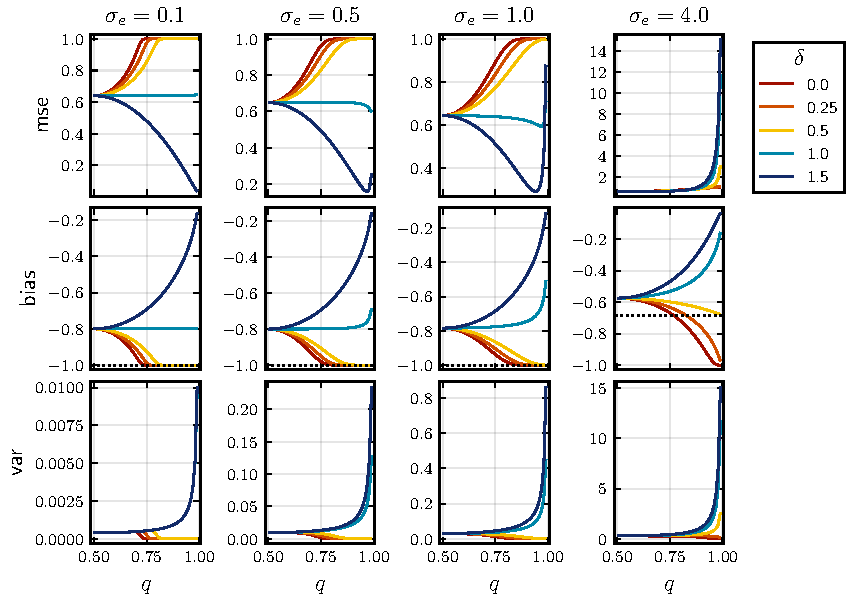
\includegraphics[]{plots/bias-var-onedim.pdf}
  \caption{%
    Bias, variance, and mean-squared error for a one-dimensional lasso problem.
    Note that \(\delta = 0\) corresponds to the case of no scaling, \(\delta = 1/2\) corresponds
    to standardization, and \(\delta = 1\) corresponds to scaling with the variance. The dotted
    lines represent the asymptotic bias of the lasso estimator in the case of \(\delta = 1/2\).
  }
  \label{fig:bias-var-onedim-lasso}
\end{figure}

\subsection{Multiple Predictors}

\begin{figure}[htpb]
  \centering
  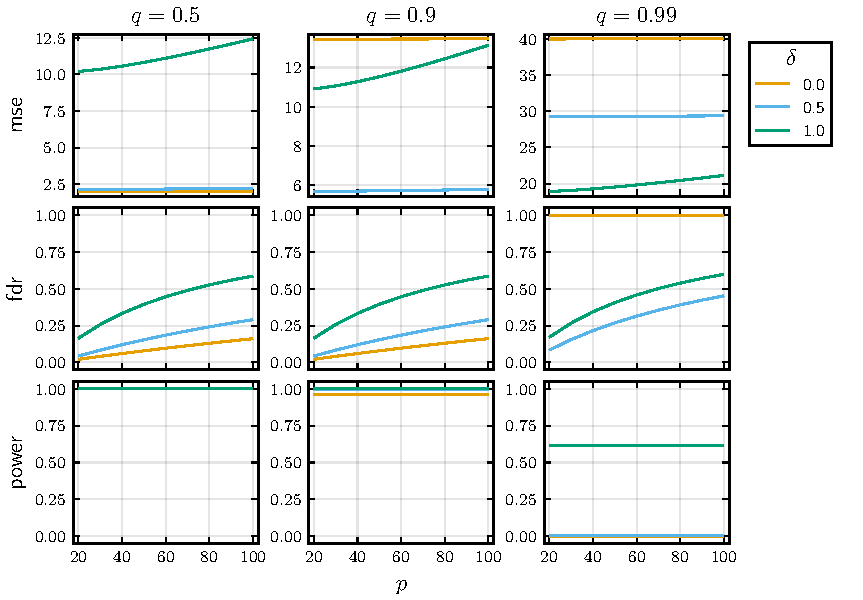
\includegraphics[]{plots/beta-bias-multidim.pdf}
  \caption{%
    Mean-squared-error, false discovery rate (FDR), and power for a lasso problem with
    \(k = 10\) true signals (nonzero \(\beta_j^*\)), varying \(p\), and \(q \in [0.5, 0.9, 0.99]\). The noise level is set at \(\sigma_\varepsilon = 1\).
  }
  \label{fig:mse-fdr-power-multidim}
\end{figure}
